\documentclass[10pt]{article}
\usepackage[utf8]{inputenc}
\usepackage{url}
\usepackage{graphicx}
\usepackage[table]{xcolor}
\usepackage{blindtext}
\usepackage{enumitem}
\usepackage{booktabs}

\begin{document}

\section{User Acceptance Testing}

User Acceptance Testing is the final stage of testing where the target user can check the system for its compliance with business requirements and allows the end user to familiarize themselves with the functionality of the system.

\subsection{Objective}
To allow the end user to run through the Avi System basing their test on the business requirements. To get feedback from the user with any questions or changes that they require and also to assess usability/intuitiveness of the system.

\subsection{Justification}
The User Acceptance testing has an important role in which the end user validates the system whether it meets the business requirements before getting deployed. 

\subsection{Participant}
This testing will be carried out by an end user (a third year Computer Science Student) that is briefed about the business requirements so that they may have knowledge about the client’s needs of the system. \\

\underline{Test Date}: 05/10/2018 \\

\underline{Tester}: Katleho Mokoena \\

\subsection{Methodology}

The user will participate in the following use cases: 

\begin{center}
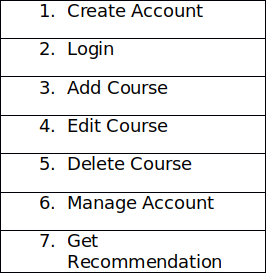
\includegraphics[width=.6\textwidth]{methodology.png}
\end{center}
\caption{\underline{Use Cases}} \\ \\

\begin{center}
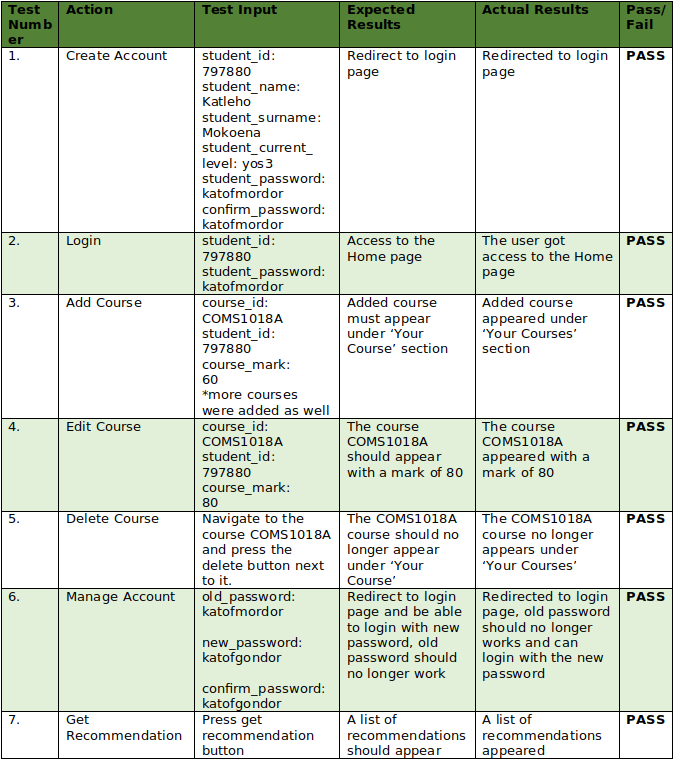
\includegraphics[width=.9\textwidth]{tester.png}
\end{center}
\caption{\underline{Actions}} \\ \\

\subsection{Results}

The user found the system easy to use and was able to perform all the tasks.

\subsection{User Acceptance Testing Summary}

Avi System passed all the user acceptance tests conducted on the specified use cases. 


\section{Unit Testing}

Unit Testing is a level of software testing where individual units or components of a software are tested. The purpose is to validate that each unit of the software performs as designed. A unit is the smallest testable part of any software. It usually has one or a few inputs and usually a single output.

Unit Testing is the first level of software testing. These tests are independent of each other.

This is achieved through white box testing which is essentially testing based on the analysis of the internal structure of the system.

\subsection{Unit Testing Benefits}

\begin{description}[font=$\bullet$~\normalfont\scshape\color{red!50!black}]

\item [] Codes are reusable.
\item [] Development is faster in the long run.
\item [] Code maintenance is easier.
\item [] Code becomes more reliable.
\item [] Debugging becomes easier.

\end{description}

In our project we used unit tests to ensure that the individual components in our code work accordingly for various possible inputs. We don’t create tests for everything, we instead focus on testing the part of our code that impact the behavior of our system.

These test cases are split into classes where a class contains test methods which test many features of one Module, for example we have a class TestUrls which tests all the possible urls which have been defined to be handled.

It’s always a good idea to test both expected and unexpected behavior. These are Commented as Test and Counter Test for most individual test cases. It is essential that both instances are considered whether they seem trivial or not. This is how our tests are conducted.

The tests are divided into two file in which one is conducted using the Django built in test modules in the file tests.py  in the main app directory and the other is conducted using Pytest modules in the test\_pytest.py file under the tests folder.

\subsection{Part One:  Using Django Test modules}

Codes extracted from tests.py.

\begin{center}
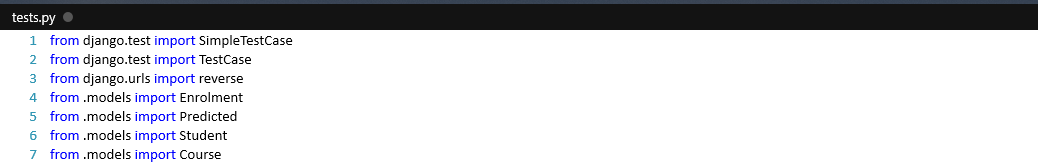
\includegraphics[width=.9\textwidth]{imports.png}
\end{center}
\caption{\underline{Imports}}
We import the models we are going to test as well. (Line 4-7)

\subsubsection{Login Page Tests}

\begin{center}
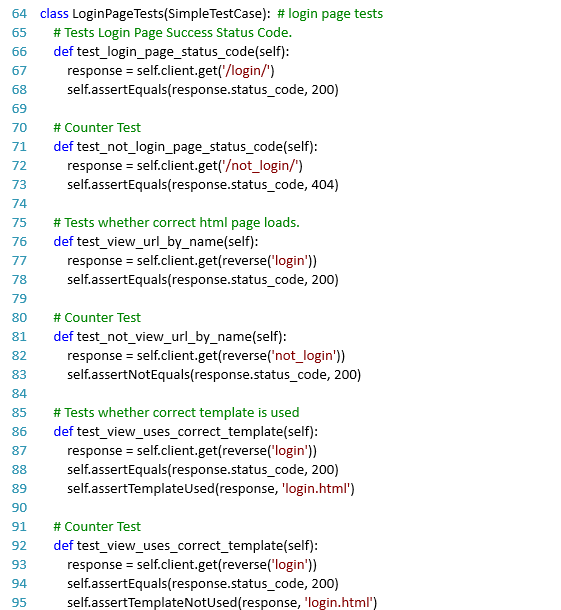
\includegraphics[width=.9\textwidth]{page_test1.png}
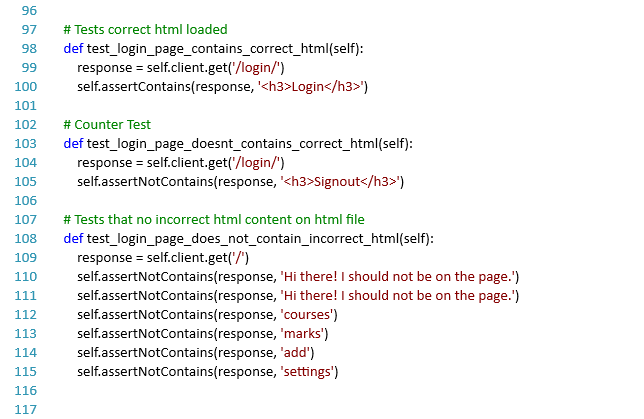
\includegraphics[width=.9\textwidth]{page_test2.png}
\end{center}
\caption{\underline{Login Page Tests}}

\begin{description}[font=$\bullet$~\normalfont\scshape\color{red!50!black}]

\item [] The login tests are defined in the class ‘LoginPageTests’ - (line 64).
\item [] The first test and counter test ensures that the login page status code is returned whenever the login url is invoked and that an error status  code is returned whenever an invalid login request (possibly due to a typing error) is passed.- (line 65-73).
\item [] The second test ensures that the correct html file is returned whenever login url is passed, the counter test ensures that ensures that its not returned anywhere else.-(lines 75-83).
\item [] The third test ensures that the correct template is used by the login url, its counter test ensures that that template is not used elsewhere. - (line 86-95).
\item [] The forth test ensures that the html file contains the word “Login” heading, its counter test ensures that the html doesn’t contain any other random headings. – (line 97-105).
\item [] The fifth test ensures that the html doesn’t contain any strings from other html files. - (line 107 - 115).

\end{description}

\subsubsection{Sign Up Page Tests}

\begin{center}
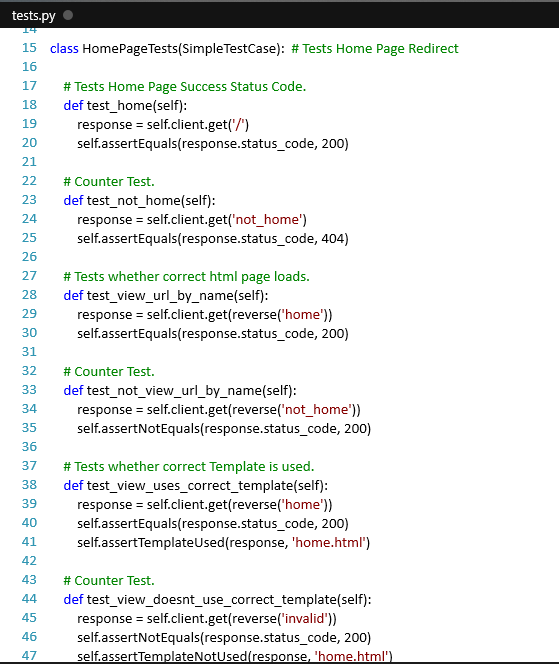
\includegraphics[width=.8\textwidth]{sign_test1.png}
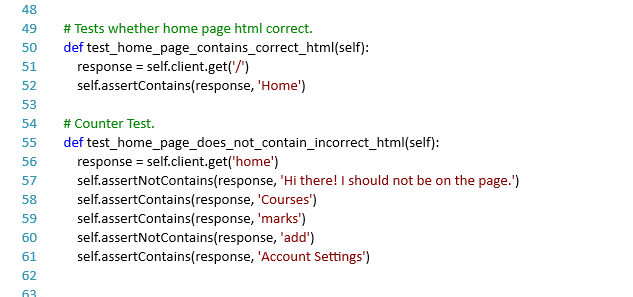
\includegraphics[width=.8\textwidth]{sign_test2.png}
\end{center}
\caption{\underline{Sign Up Page Tests}}

\begin{description}[font=$\bullet$~\normalfont\scshape\color{red!50!black}]

\item [] The HomePage tests are defined in the class ‘HomePageTests’ - (line 15).
\item [] The first test and counter test ensures that the home page status code is returned whenever the home url is invoked and that an error status  code is returned whenever an invalid home request (possibly due to a typing error) is passed.- (line 17-25).
\item [] The second test ensures that the correct html file is returned whenever home url is passed, the counter test ensures that ensures that its not returned anywhere else.-(lines 27-35).
\item [] The third test ensures that the correct template is used by the home url, its counter test ensures that that template is not used elsewhere. - (line 37-47).
\item [] The fourth test ensure that the correct home url is loaded and returned.

\end{description}

\subsubsection{Model Tests}

\begin{center}
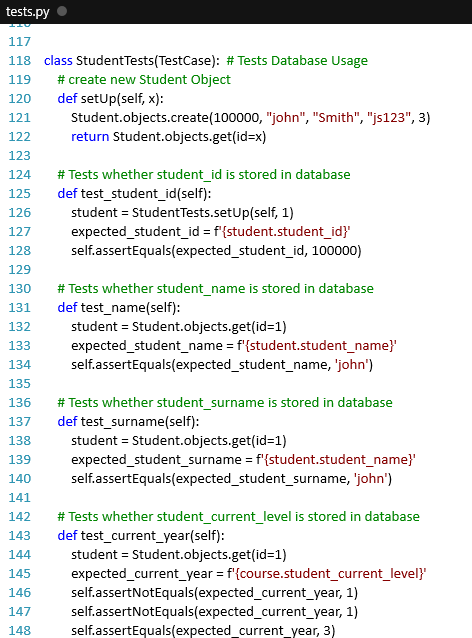
\includegraphics[width=.8\textwidth]{model_1.png}
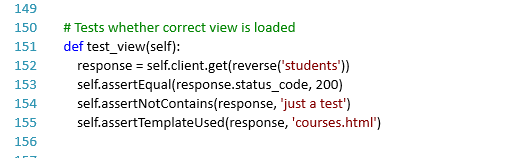
\includegraphics[width=.8\textwidth]{model_2.png}
\end{center}
\caption{\underline{Model Tests}}

\begin{description}[font=$\bullet$~\normalfont\scshape\color{red!50!black}]

\item [] The Student Model tests are defined in the class ‘StudentTests’ - (line 118).
\item [] The first test ensures that the student\_id is stored in the database. – (line 125-128).
\item [] The second test ensures that the student\_name is stored in the database. – (line 131-134).
\item [] The third test ensures that the student\_surname is stored in the database. – (line 137-140).
\item [] The fourth test ensures that the student\_current\_level is stored in the database. – (line 143-148).
\item [] The fifth test ensures that the correct view is loaded.- (line 151-156).

\end{description}

\begin{center}
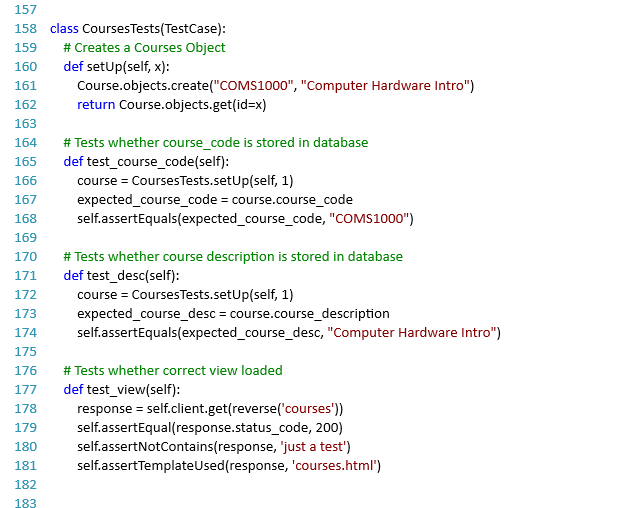
\includegraphics[width=.9\textwidth]{pc1.png}
\end{center}

\begin{description}[font=$\bullet$~\normalfont\scshape\color{red!50!black}]

\item [] The Course Model tests are defined in the class ‘CourseTests’ - (line 158).
\item [] The first test ensures that the course\_code is stored in the database. – (line 165-168).
\item [] The second test ensures that the course\_desc is stored in the database. – (line 171-174).
\item [] The third test ensures that the correct view is loaded.- (line 177-181).
\end{description}

\begin{center}
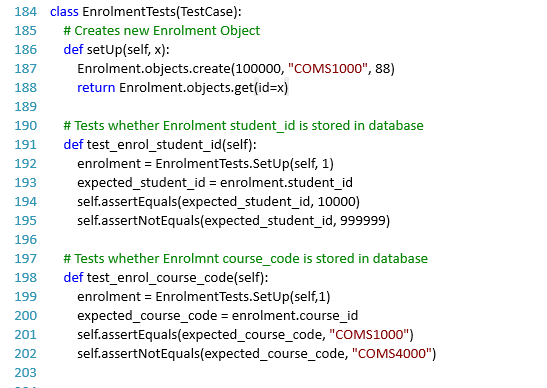
\includegraphics[width=.9\textwidth]{pc2.png}
\end{center}

\begin{description}[font=$\bullet$~\normalfont\scshape\color{red!50!black}]

\item [] The Enrolment Model tests are defined in the class ‘EnrolmentTests’ - (line 184).
\item [] The first test ensures that the student\_id (foreign key) is stored in the database. – (line 191-195).
\item [] The second test ensures that the course\_code is stored in the database. – (line 198-202).

\end{description}

\begin{center}
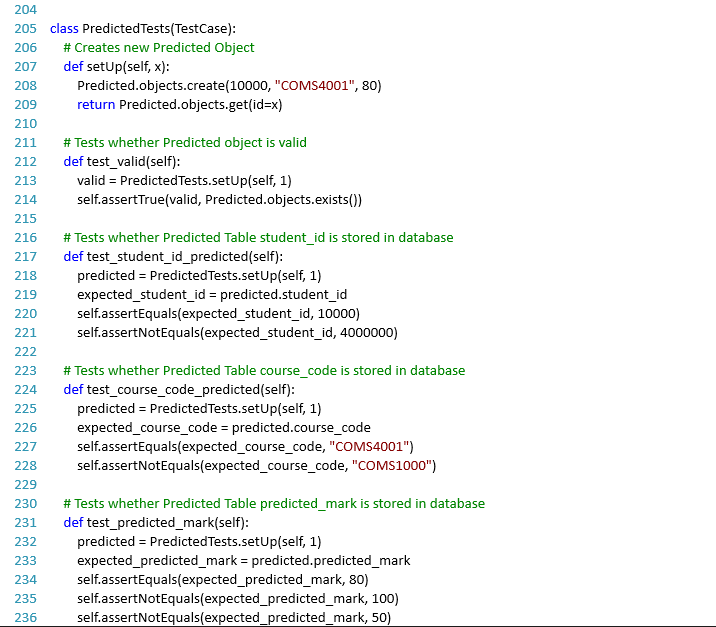
\includegraphics[width=.9\textwidth]{pc3.png}
\end{center}

\begin{description}[font=$\bullet$~\normalfont\scshape\color{red!50!black}]

\item [] The Predicted Model tests are defined in the class ‘PredictedTests’ - (line 184).
\item [] The first test ensures that the predicted object which was created is valid.- (line 212-214).
\item [] The second test ensures that the student\_id (foreign key) is stored in the database. – (line 217-220).
\item [] The third test ensures that the course\_code(foreign key) is stored in the database. – (line 224-228).
\item [] The fourth test ensures that the predicted\_mark is stored in the database. – (line 231-236).

\end{description}


\end{document}